\documentclass{article}[a4paper]

\usepackage{subfigure}
\usepackage{graphicx}
\usepackage{amsmath}

\begin{document}

\section*{Introduction}

Podvodni habitat ostvaruje vezu s brodom pomoću ultrazvučnih hidrofona postavljenih na vrh habitata. Kako bi se povećao domet ultrazvučne komunikacije, više hidrofona se može povezati u beamforming sustav. Za to je na vrhu habitata predvidjena pravokutna ravna površina veličine 1 m x 1 m, postavljena u y-z ravninu referentnog koordinatnog sustava, kako je prikazano na slici \ref{fig:coord}.
\begin{figure}[h!]
   \centering
   
\includegraphics[width=0.4\textwidth]{coord.png}
   \caption{Reference coordinate system with available beamformer area}
   \label{fig:coord}
\end{figure}

Hidrofon radi u frekvencijskom rasponu od 20 kHz do 90 kHz, a za komunikaciju je odabrana frekvencija nosioca od 30 kHz. Smatrajte da je signal uskopojasan. Hidrofon ima kosinusni dijagram zračenja opisan formulom
\[ D(\phi,\theta) = \cos^2(\theta) \]
gdje je $\phi$ kut azimuta, a $\theta$ kut elevacije. Dijagram zračenja u referentnom koordinatnom sustavu je prikazan slikom \ref{fig:hydrophone}.
\begin{figure}[h!]
   \centering
   \subfigure[3D view]{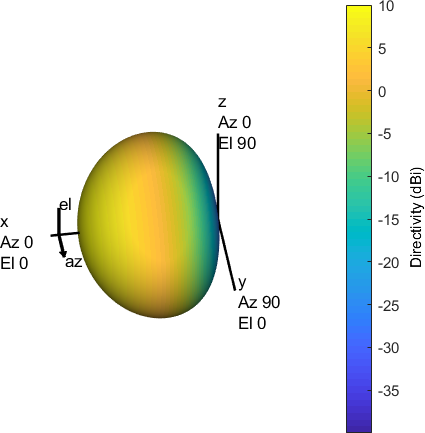
\includegraphics[width=0.415\textwidth]{hydrophone_3d.png}}
   \hfill
   \subfigure[Azimuth cut at 0deg]{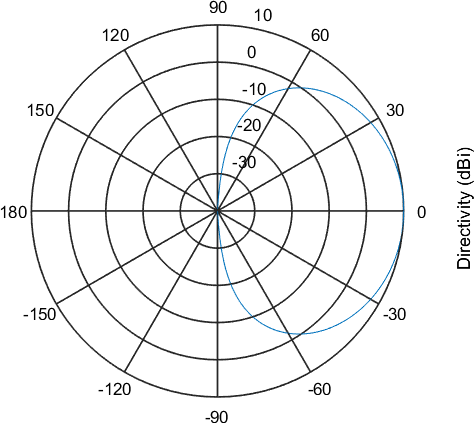
\includegraphics[width=0.45\textwidth]{hydrophone_cut.png}}
   \caption{Farfield of a hydrophone element}
   \label{fig:hydrophone}
\end{figure}
Hidrofoni su fizički kružni, promjera 5 cm. Svi hidrofoni antenskog sustava postavljaju se s maksimumom zračenja u zenit, tj. okomito na površinu mora. S druge strane, brod raspolaže s jednim hidrofonom montiranim na trup broda i okrenutim u nadir, tj. okomito na morsko dno. Brod se nalazi u dalekom polju antenskog sustava.

Smatrajte da se komunikacija odvija u Jadranskome moru, prosječnog saliniteta 28\% i u temperaturi mora od 20deg.

\pagebreak

\section*{Task 1}

Potrebno je dizajnirati linearni antenski niz za postizanje najboljeg linka izmedju dviju stanica. Zadana su tri scenarija. Obratite pozornost na koordinatni sustav. Kut elevacije se promatra od normale antenskog sustava.
\begin{description}
	\item[Scenario 1] Brod se naalzi točno iznad antenskog sustava.
	\item[Scenario 2] Brod se nalazi iznad uzdužne osi antenskog sustava, na elevaciji od 30 stupnjeva.
	\item[Scenario 3] Brod se nalazi iznad uzdužne osi antenskog sustava, na elevaciji od 60 stupnjeva.
	\item[Scenario 4] Brod se nalazi iznad uzdužne osi antenskog sustava, na elevaciji od 70 stupnjeva.
\end{description}
\subsection*{Scenarij 1}

\begin{figure}[h!]
   \centering
   \subfigure[Scenario 1]{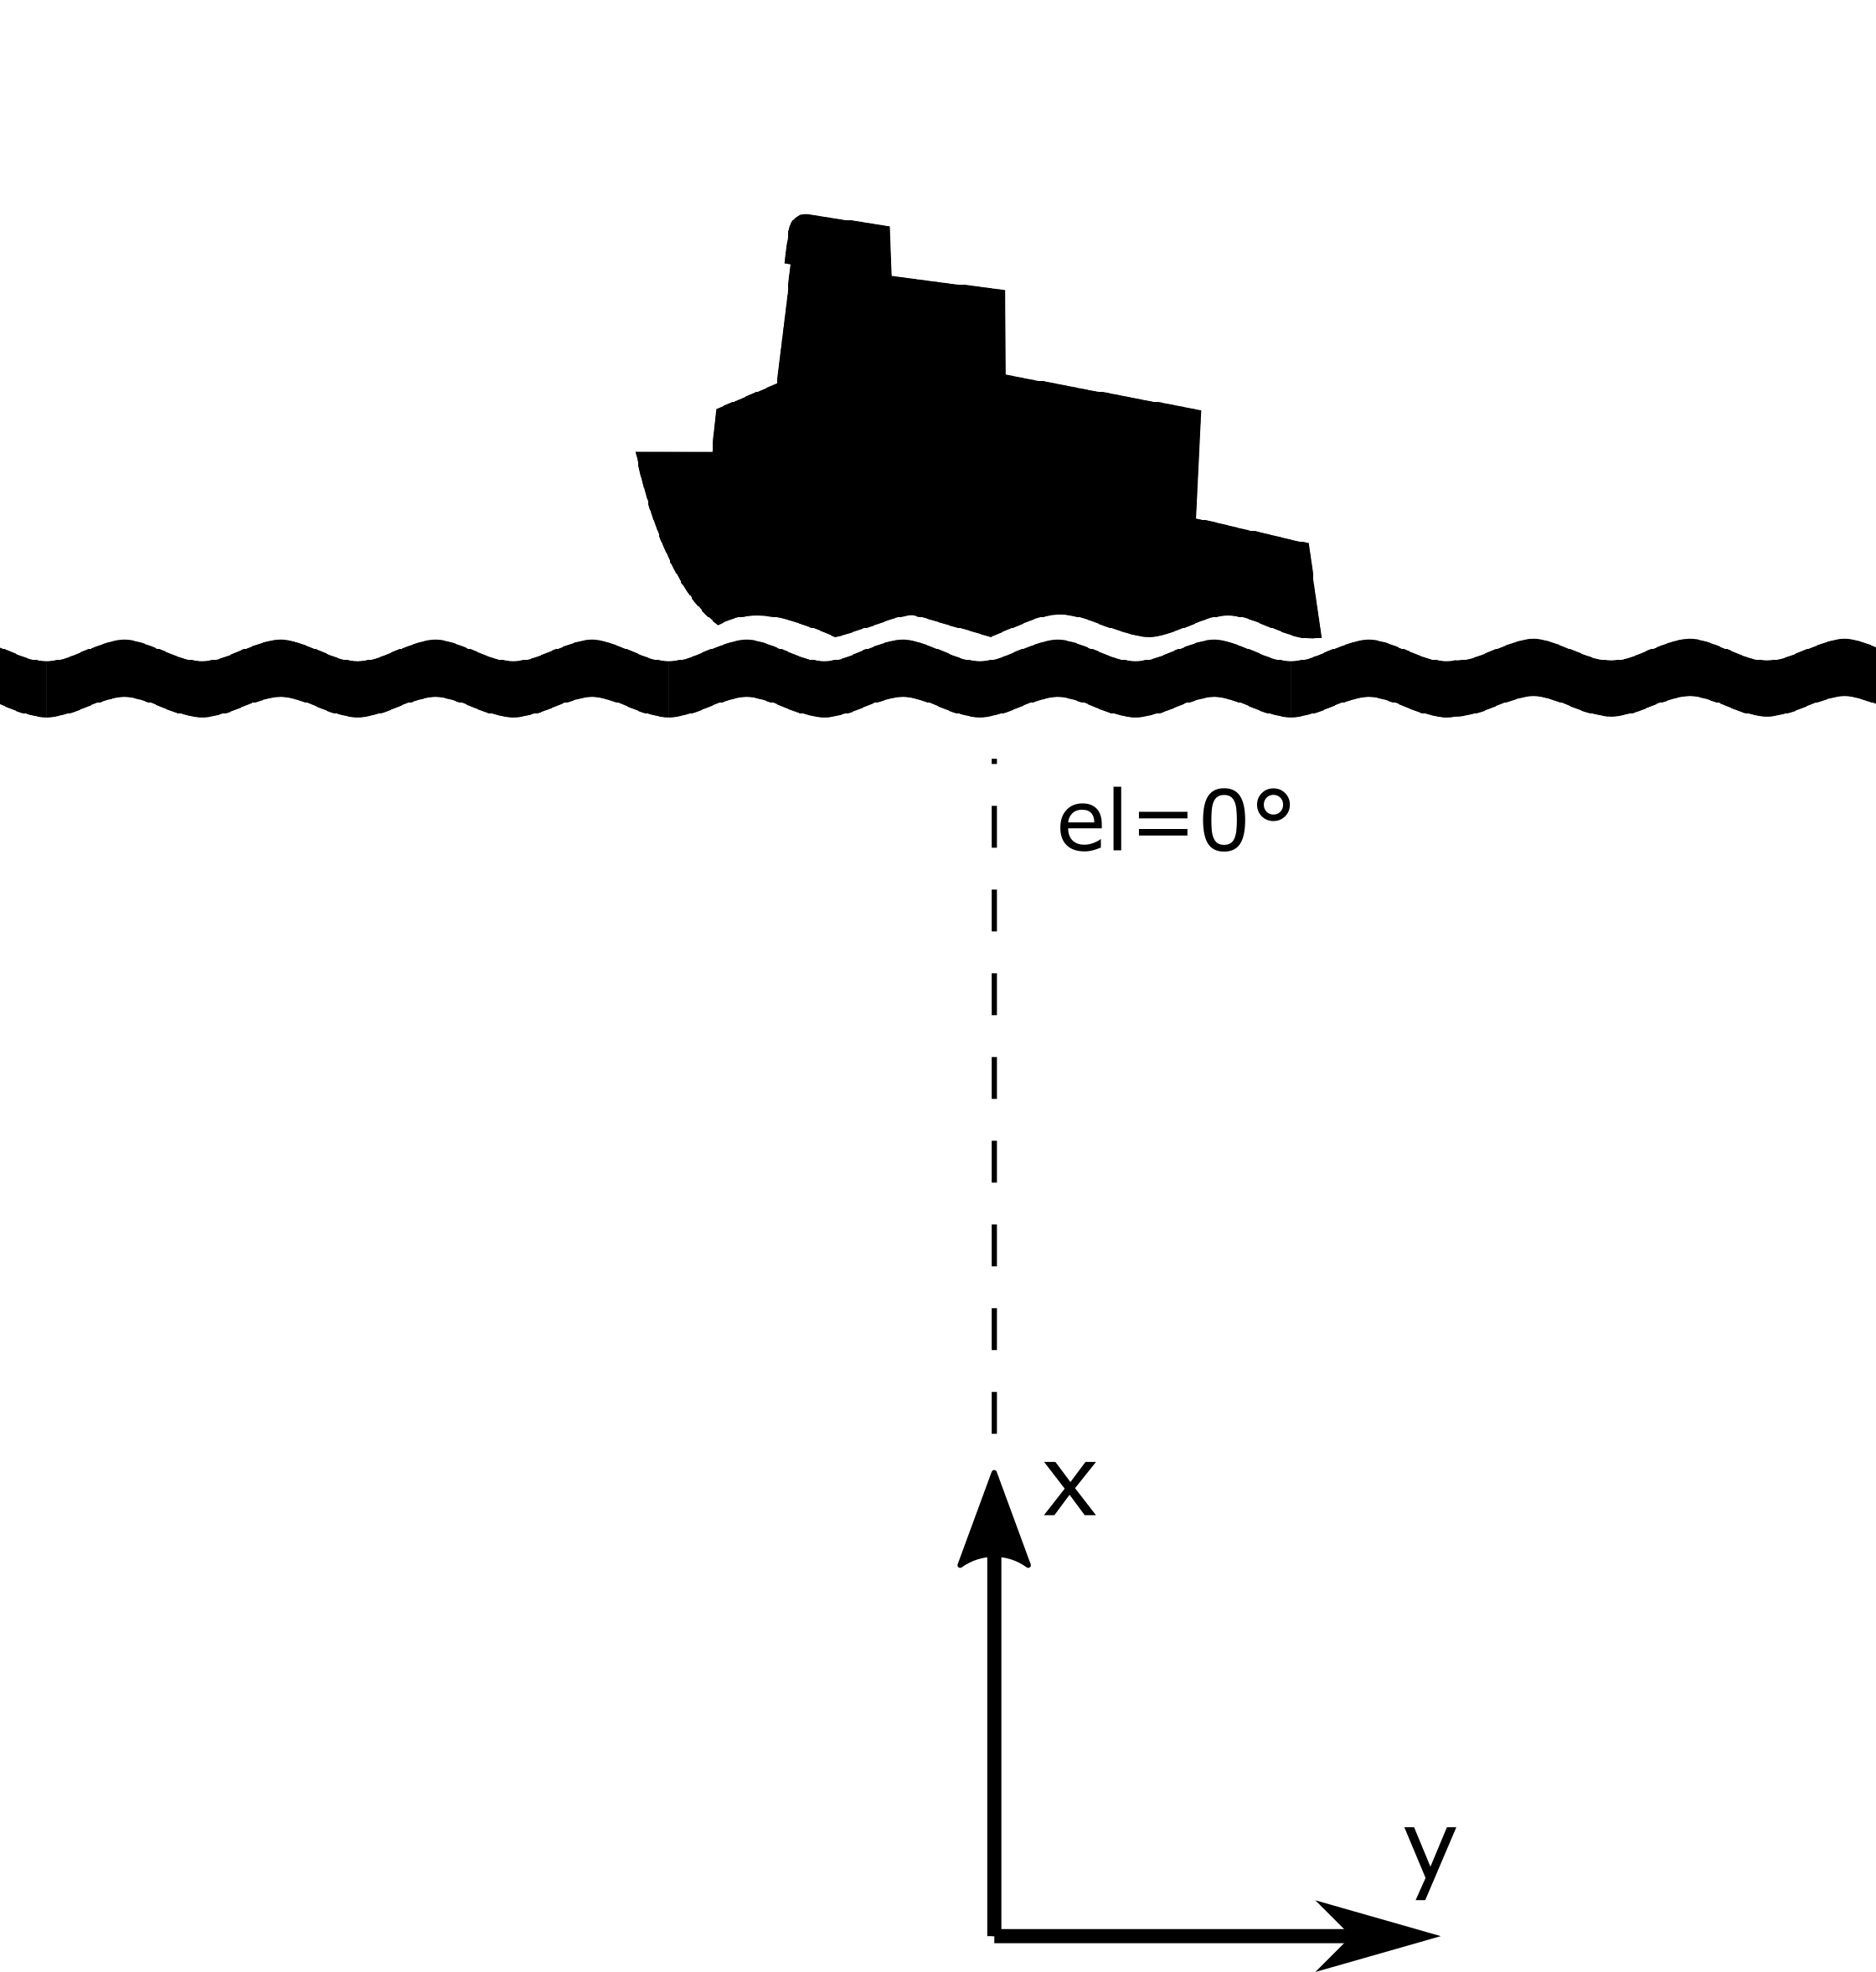
\includegraphics[width=0.45\textwidth]{scenario1.png}}
   \hfill
   \subfigure[Scenario 2]{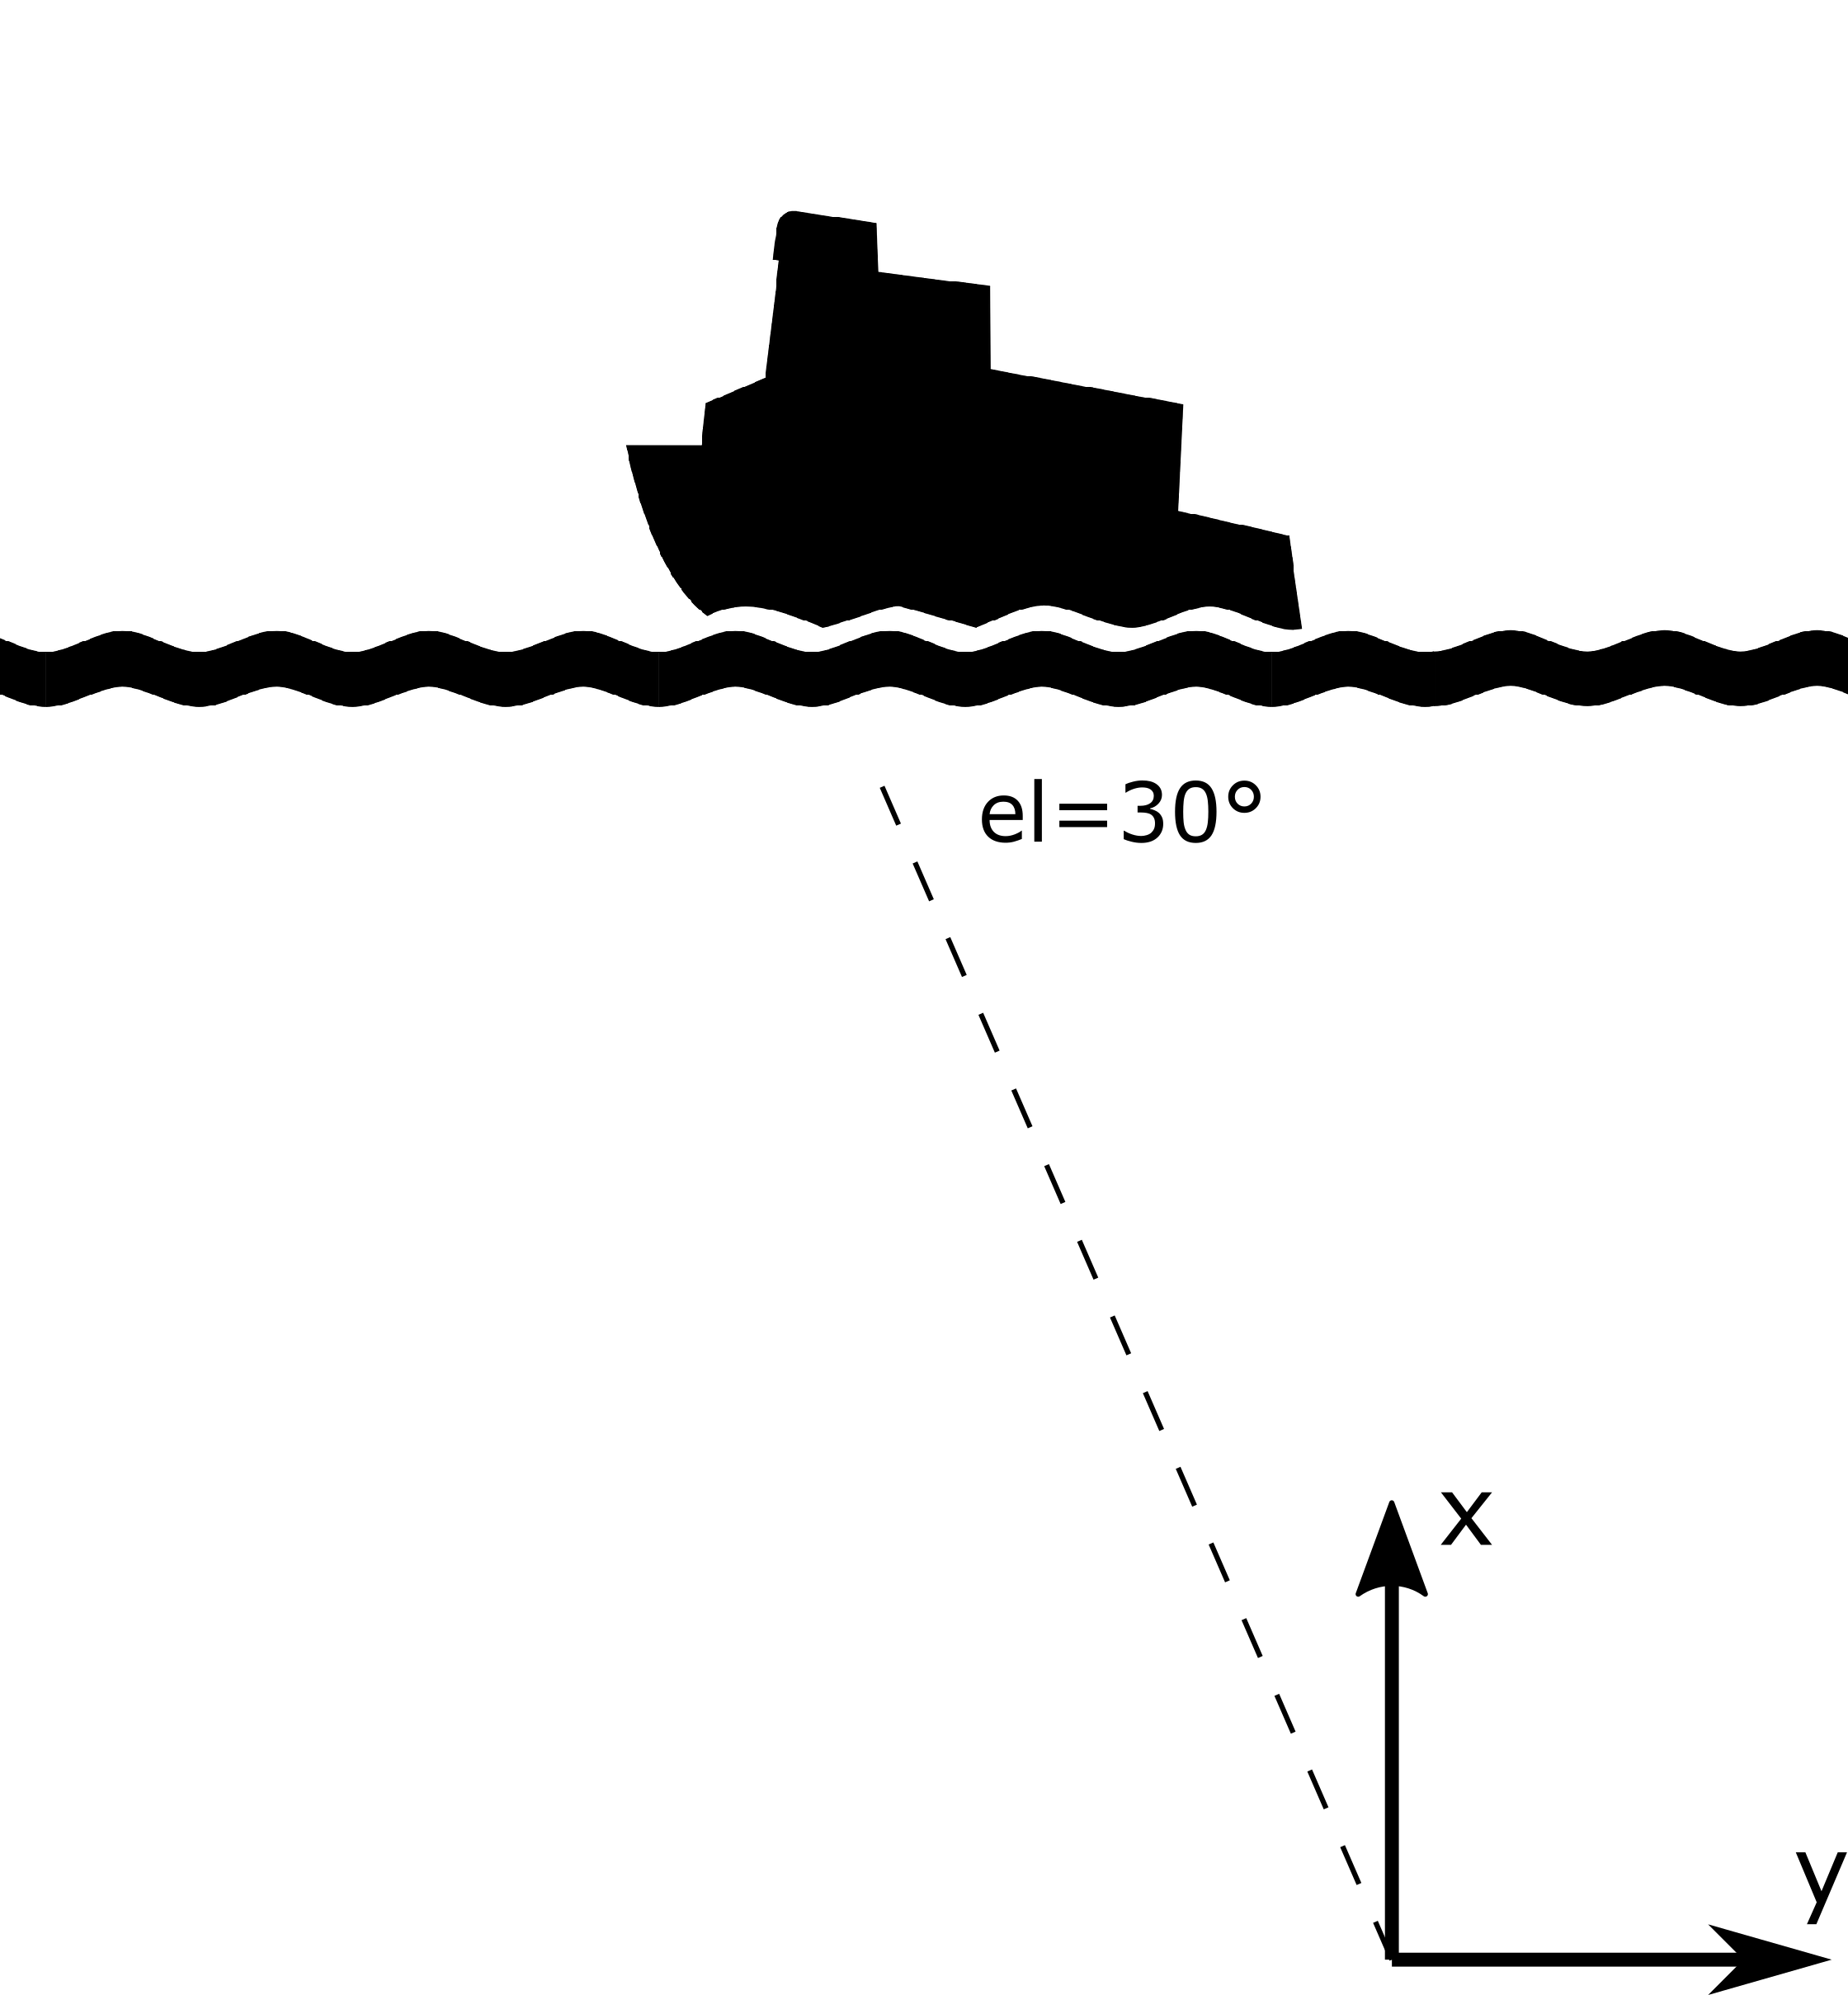
\includegraphics[width=0.45\textwidth]{scenario2.png}}
   \\
   \subfigure[Scenario 3]{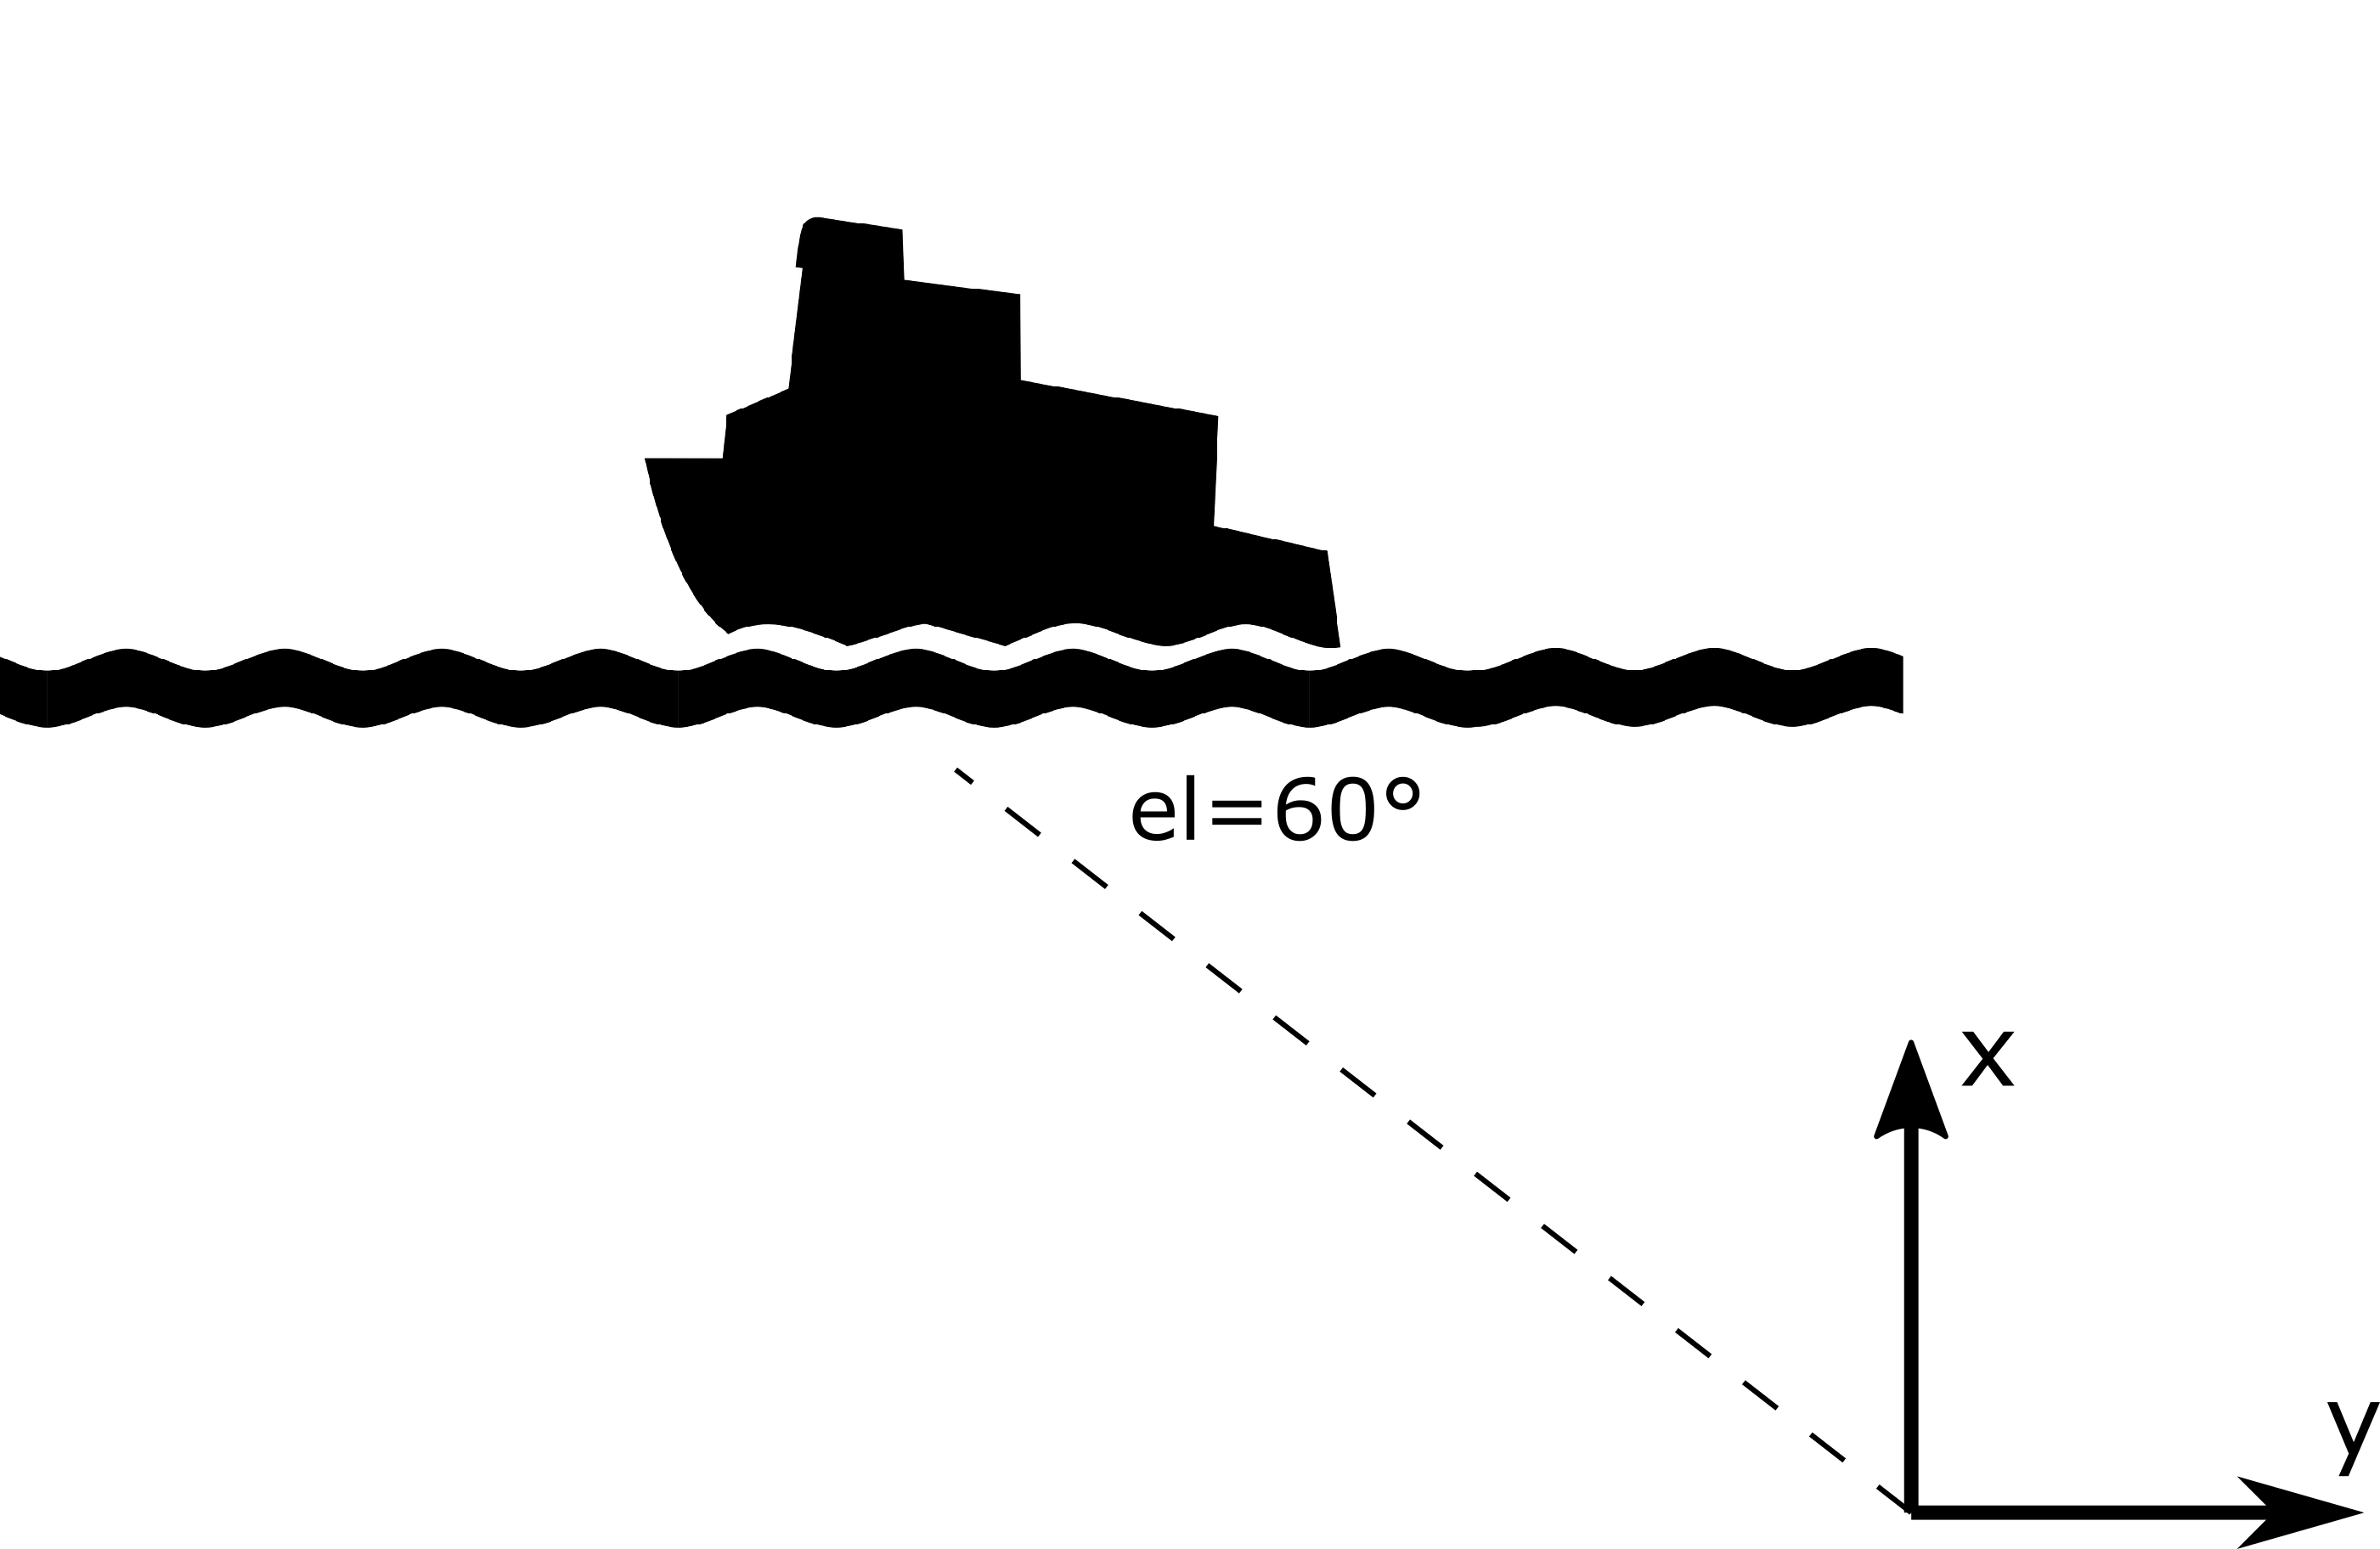
\includegraphics[width=0.45\textwidth]{scenario3.png}}
   \hfill
   \subfigure[Scenario 1]{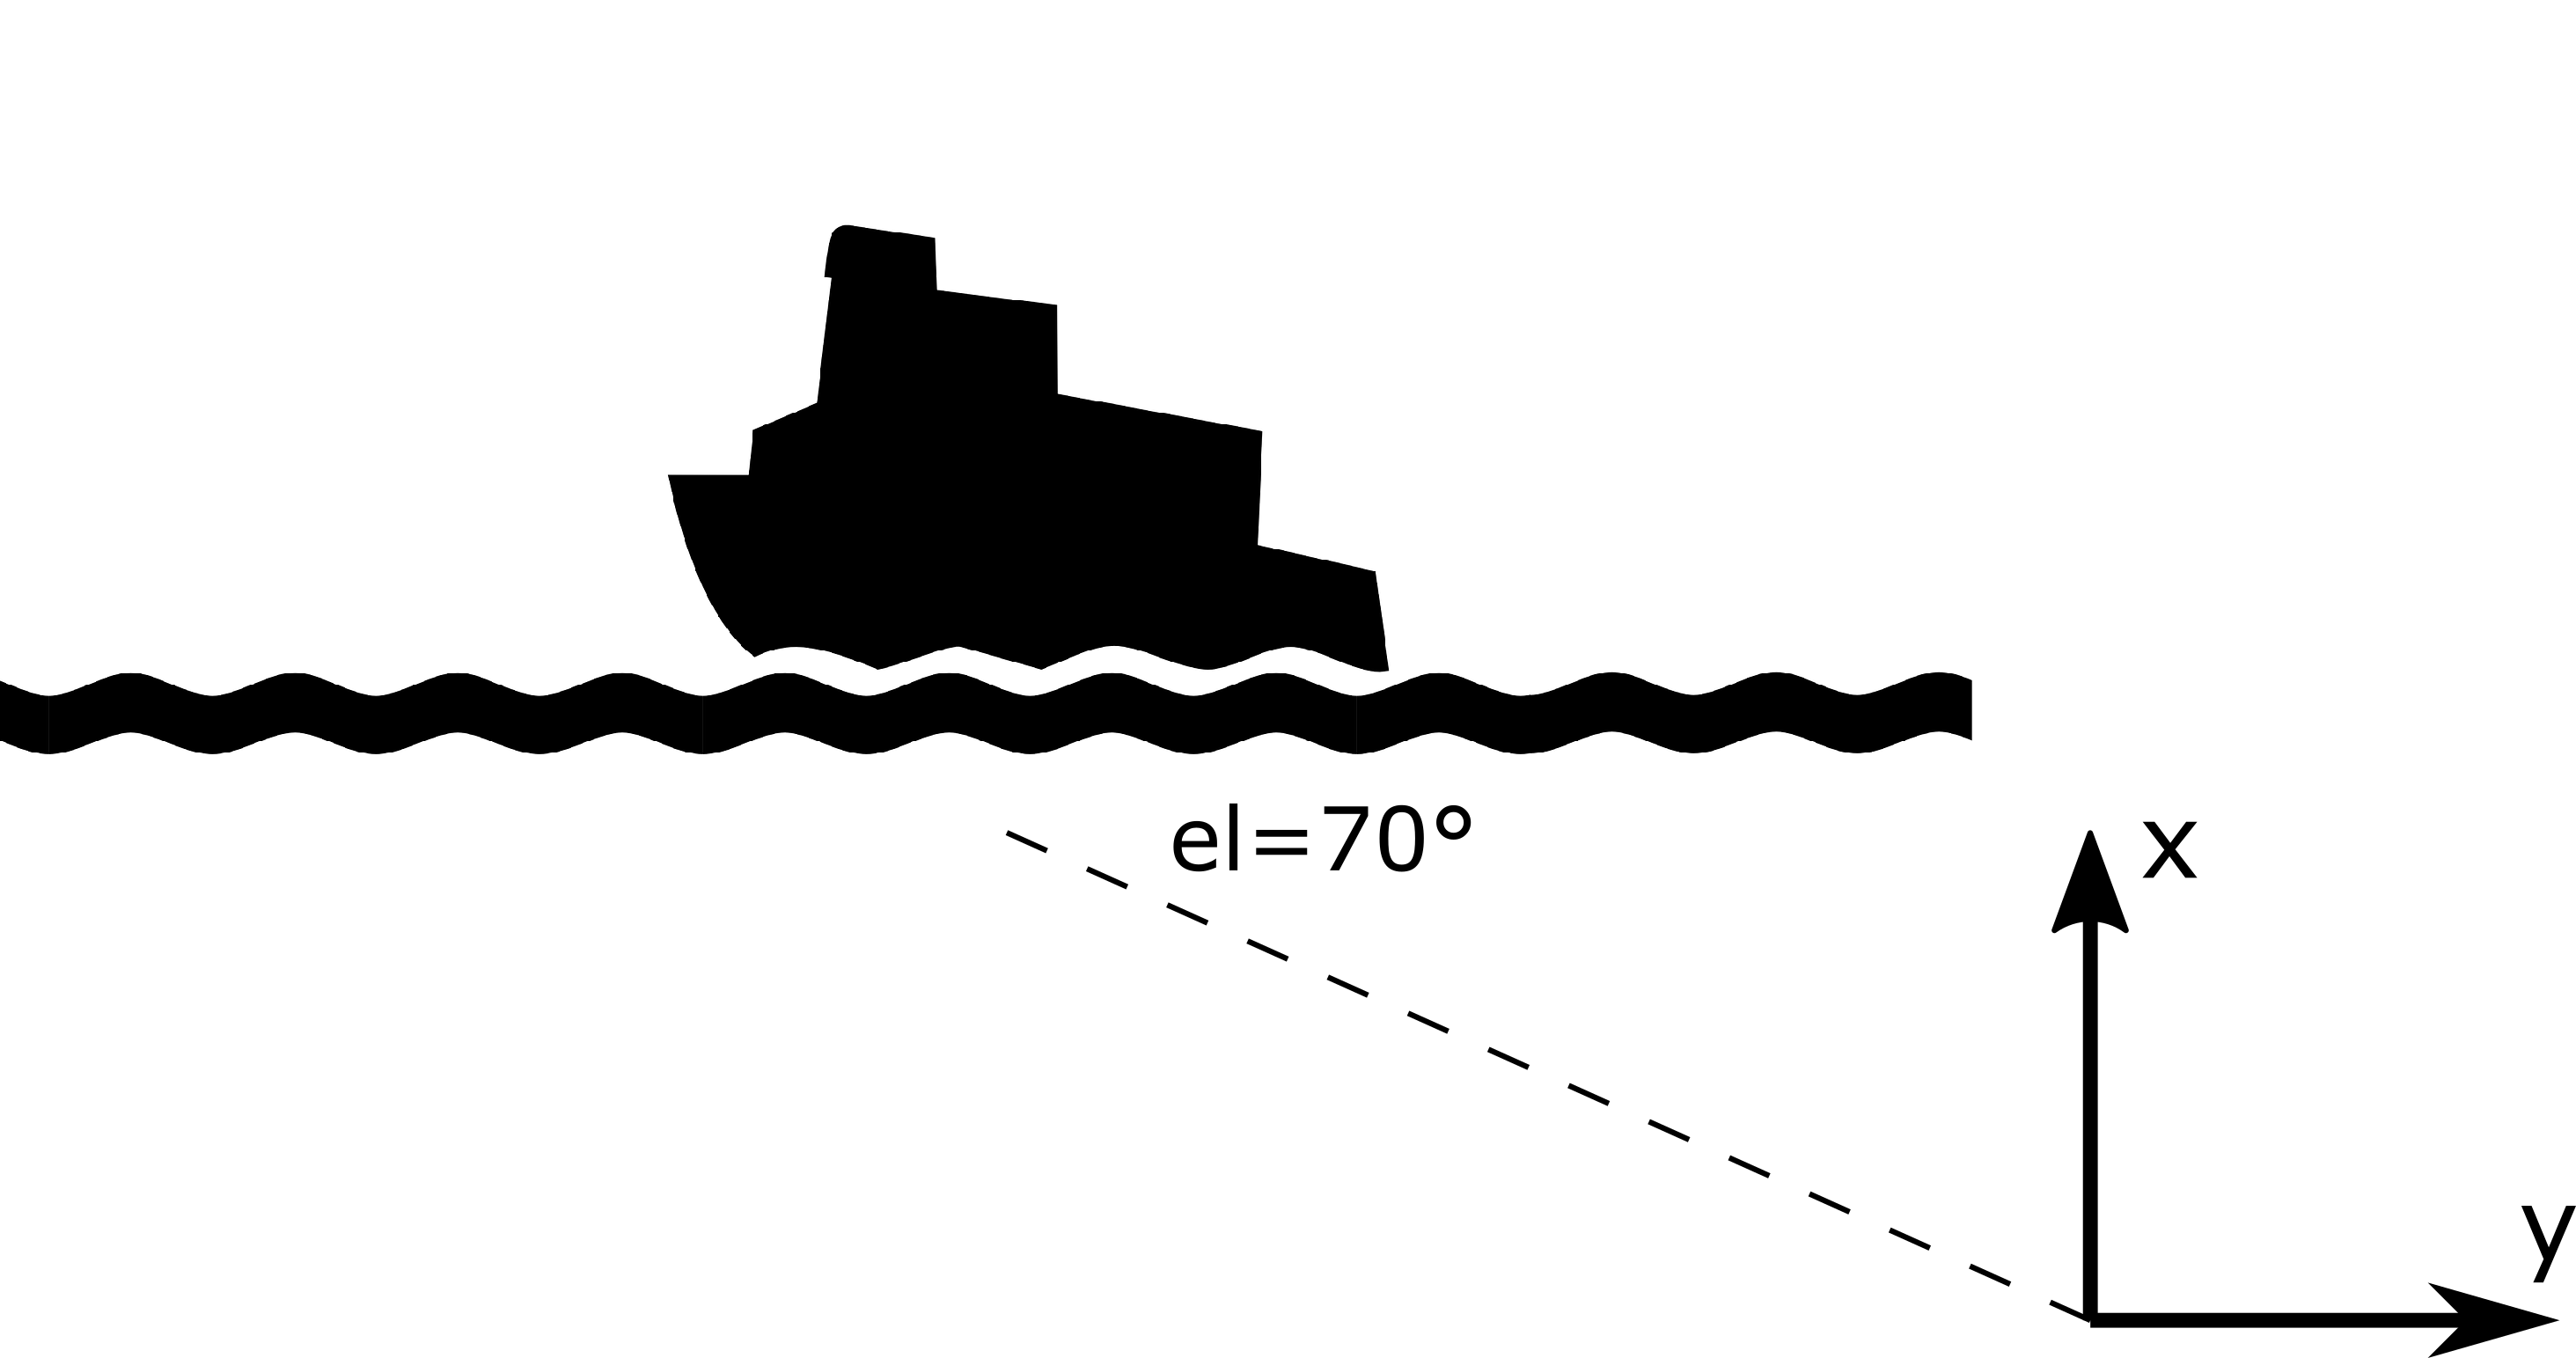
\includegraphics[width=0.45\textwidth]{scenario4.png}}
   \caption{Scenarios for Task 1}
\end{figure}

Dizajnirajte jedan linearni antenski niz koji će raditi dobro za sva 4 scenarija. Antenski niz je definiran y koordinatom svakog antenskog elementa. Broj elemenata je proizvoljan, uz ograničenja zadana u uvodnom dijelu zadatka.

Za svaki od 4 scenarija odredite težinske faktore koji se dovode na svaki antenski element kako bi se postigao najbolji mogući beamforming za taj scenarij.

\subsection*{Output data}

\begin{description}
	\item[task1\_elements.csv] \,\\ Datoteka sadrži jednodimenzionalni niz koji označava pozicije antenskog elementa na y osi
	\item[task1\_scenarioX.csv] \,\\ Datoteka sadrži jednodimenzionalni niz kompleksnih brojeva koji predstavljaju kompleksnu težinu svakog antenskog elementa, respektivno prema podacima iz task1\_elements.csv. Duljina niza jednaka je broju elemenata. Svi brojevi se nalaze unutar jedinične kružnice.
\end{description}

\subsection*{Scoring}

Za sve zadane scenarije evaluira se antenski sustav koji ste dizajnirali. U prva tri scenarija, bodovi se dodjeljuju za usmjerenost koju antenski sustav ostvaruje u smjeru broda.
Ako se brod nalazi u glavnoj latici antenskog niza, tada tim dobiva bodove u iznosu najveće usmjerenosti glavne latice. Ako se brod nalazi u sekundarnoj latici najveće usmjerenosti, tada tim dobiva bodove prema formuli
\[ D_\textrm{target} - \dfrac{\varDelta \phi}{10} \]
gdje je $D_\textrm{target}$ usmjerenost u smjeru broda, a $\varDelta \phi$ kutni razmak izmedju smjera najvećeg zračenja i broda, u stupnjevima. Smatra se da je brod unutar latice ako je usmjerenost u njegovom smjeru unutar 6 dB usmjerenosti iste latice.

U scenariju 4, dizajnirani antenski sustav se evaluira sa težinskim faktorima koje izračunate, te usporedjuje usmjerenost koju antenski sustav ostvaruje u smjeru broda u odnosu na usmjerenost koju bi ostvario u slučaju uniformne pobude. Najveći broj bodova koji se u ovom scenariju može ostvariti je 15.

Antenski sustav koji se sastoji od samo jednog elementa ne dobiva bodove ni u kojem scenariju. Antenski niz koji ima negativno usmjerenje u smjeru broda ne dobiva bodove ni u kojem scenariju. Iznosi usmjerenosti evaluiraju se u jedinicama dBi. Timovi ne mogu dobiti negativni broj bodova.

Nakon evaluacije svih timova za oba zadatka, ukupan broj bodova svakog tima se normira na najbolji tim. Dakle, najbolji tim dobiva 50 bodova, a bodovi ostalih timova se linearno skaliraju prema njima.

\end{document}